\section{Ptolemy and The Celestial Circles: When Geometry Became a Calculator}

\subsection{From Harmony to Heuristics: When Math Got Down to Earth}

The Pythagoreans dreamed of a cosmos that resonated like a lyre — where planets sang and proportions whispered secrets of divine order. But while they listened for music in the stars, later thinkers began asking a more pragmatic question: \textit{Where exactly is Mars going to be next Tuesday?}

Enter Claudius Ptolemy.

Where the Pythagoreans sought meaning, Ptolemy sought measurement. He kept the circular perfection, the geocentric certainty, and the divine symmetry — but turned these ideals into instruments of calculation.

Instead of chords on strings, he used chords in circles. Instead of mystical harmony, he gave us geometric astronomy.

\begin{figure}[H]
    \centering
    \begin{tikzpicture}[>=latex]
      % === Chord on a string ===
      \begin{scope}[shift={(-4,0)}]
        % the “string”
        \draw[-] (-2,0) -- (2,0);
        % endpoints A and B
        \node[fill=black, circle, inner sep=1.5pt] (A) at (-1.5,0) {};
        \node[fill=black, circle, inner sep=1.5pt] (B) at (1.5,0) {};
        % the chord
        \draw[very thick] (A) -- (B);
        % labels
        \node[below=4pt] at (0,0) {Chord on a string};
        \node[above] at (A) {A};
        \node[above] at (B) {B};
      \end{scope}
  
      % === Chord in a circle ===
      \begin{scope}[shift={(4,0)}]
        % the circle
        \draw (0,0) circle (2cm);
        % two points C and D on the circumference
        \coordinate (C) at (60:2cm);
        \coordinate (D) at (-10:2cm);
        \node[fill=black, circle, inner sep=1.5pt] at (C) {};
        \node[fill=black, circle, inner sep=1.5pt] at (D) {};
        % the chord
        \draw[very thick] (C) -- (D);
        % labels
        \node[right=4pt] at ($(C)!0.5!(D)$) {Chord in a circle};
        \node[above] at (C) {C};
        \node[below right] at (D) {D};
      \end{scope}
    \end{tikzpicture}
    \caption{Comparison: a straight‐line “chord” on a string (left) versus a circular chord (right).}
\end{figure}
  

And so began the age of epicycles.

Ptolemy’s model wasn’t just about celestial prediction; it was about \emph{preserving a metaphysical worldview}. His system endured for over a thousand years, not because it was the most accurate, but because it was philosophically elegant. It kept the cosmos ordered, the Earth central, and the heavens divine.

But when you looked at the planets, they defied those expectations. They sped up, slowed down, and sometimes even moved backwards (retrograde motion). Ptolemy reconciled this by constructing a system of \textbf{epicycles and deferents} — circles moving on other circles — all governed by geometric rules.

\begin{figure}[H]
    \centering
    \begin{tikzpicture}[scale=1]
      % Earth at center
      \node[fill=black, circle, inner sep=1.5pt, label=below:Earth] (C) at (0,0) {};
  
      % Deferent circle
      %\draw (0,0) circle (2cm) node[above right=2pt] {Deferent};
      \draw (0,0) circle (2cm);
  
      % Epicycle center on deferent
      \coordinate (D) at (45:2cm);
      \node[fill=black, circle, inner sep=1pt] at (D) {};
      %\node[right=3pt] at (D) {Epicycle center};
  
      % Epicycle circle
      %\draw (D) circle (0.7cm) node[right=4pt] {Epicycle};
      \draw (D) circle (0.7cm);
  
      % Planet position on epicycle
      \coordinate (P) at ($(D)+(-30:0.7cm)$);
      \node[fill=black, circle, inner sep=1.5pt, label=below right:Planet] at (P) {};
  
      % Motion arrows
      %\draw[->, thin]
      %  (30:2cm) arc (30:80:2cm) node[midway, right] {Deferent motion};
      %\draw[->, thin]
      %  ($(D)+(-20:0.7cm)$) arc (-20:20:0.7cm) node[midway, above] {Epicycle motion};
    \end{tikzpicture}
    \caption{Ptolemaic geocentric model: a planet on an epicycle rolling around the deferent.}
\end{figure}

To compute planetary positions, he used:

\begin{itemize}
    \item Chords of central angles in a circle,
    \item Geometric transformations of rotating systems,
    \item Interpolation from chord tables — not modern trigonometric functions.
\end{itemize}


\begin{tcolorbox}[colback=blue!5!white, colframe=blue!50!black, breakable,
    title={Historical Sidebar: Why Ptolemy Used Chords in Circles — The Legacy of Euclid and Hipparchus}]
    
    Before Ptolemy, two figures laid the mathematical foundation for celestial calculation:

    \medskip

    \begin{itemize}
        \item \textbf{Euclid}: the authore of \textit{Elements} which codified geometry as a rigorous, deductive system 
        \item \textbf{Hipparchus}: the astronomer who first applied geometry to the heavens with systematic precision
    \end{itemize}
    
    \medskip
    
    Euclid gave the tools: lines, angles, circles, and theorems.  

    \medskip

    Hipparchus gave the application: using those tools to measure the sky.

    \medskip
    
    In particular, Hipparchus introduced the idea of using \textbf{chords of a circle} to compute angular distances.  
    %Without trigonometric functions like sine or cosine, he created a table of chord lengths: for a given central angle \( \theta \), what is the straight-line segment connecting the two points on a circle’s circumference?
    
    %\[
    %\text{Chord}(\theta) = 2R \cdot \sin\left(\frac{\theta}{2}\right)
    %\]
    
    %Though Ptolemy would not have expressed it this way, 

    \medskip
    
    Potolemy built upon this method in the \textit{Almagest}, extending and refining Hipparchus’s chord tables.
    
    \medskip
    
    Why chords in circles instead of chords on strings?

    \medskip
    
    Because for Ptolemy —-- and the Hellenistic tradition —-- the circle wasn’t just a shape.  

    \medskip
    It was the \textbf{perfect form} for perfect motion.  And Euclidean geometry, especially when systematized in astronomical models by Hipparchus, gave him the mathematical framework to turn cosmic harmony into celestial computation.
    
    
\end{tcolorbox}



\subsection{The Chord Table: A Trigonometric System Without Trig}

Ptolemy tabulated the lengths of \textbf{chords} — straight lines connecting the endpoints of arcs — for angles from \( 0^\circ \) to \( 180^\circ \), in half-degree steps, using a fixed radius of \( R = 60 \) units, following Babylonian sexagesimal conventions.

\medskip

\begin{figure}[H]
    \centering
    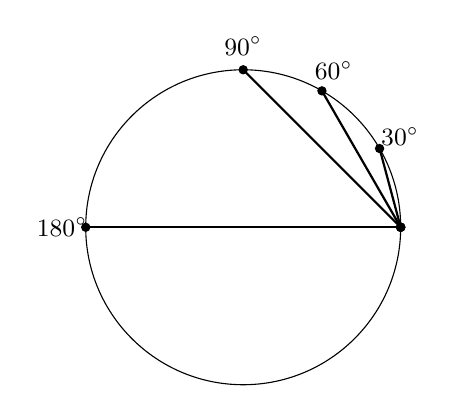
\begin{tikzpicture}[scale=1, every node/.style={font=\small}]
      % Draw the circle
      \draw (0,0) circle (2cm);
  
      % Place the 8 defining points on the circumference
      \foreach \pt/\ang in {
        A/0,  B/30,
        C/0,  D/60,
        E/0,  F/90,
        G/0, H/180
      }{
        \coordinate (\pt) at (\ang:2cm);
        \node[fill=black, circle, inner sep=1.2pt] at (\pt) {};
      }
  
      % Draw the four chords
      \draw[thick] (A) -- (B);
      \draw[thick] (C) -- (D);
      \draw[thick] (E) -- (F);
      \draw[thick] (G) -- (H);
  
      % Degree‐labels just outside the circle
      \node at (30:2.3cm)  {$30^\circ$};
      \node at (60:2.3cm)  {$60^\circ$};
      \node at (90:2.3cm)  {$90^\circ$};
      \node at (180:2.3cm) {$180^\circ$};
    \end{tikzpicture}
    \caption{Chords for 30°, 60°, 90° and 180°, with degree labels placed outside the circle.}
\end{figure}

\medskip

This system predates modern sine and cosine. Instead of projecting vertical segments, the Greeks computed the actual linear length of the arc’s chord, relying on proportions, geometric constructions, and Pythagorean relationships.

\medskip

\begin{table}[H]
\centering
\renewcommand{\arraystretch}{1.5}
\begin{tabular}{|c|p{8cm}|}
\hline
\textbf{Angle \( \theta \)} & \textbf{Chord Length (in terms of geometric construction)} \\
\hline
\( 0^\circ \) & Zero length — endpoints coincide. \\
\hline
\( 30^\circ \) & Construct an equilateral triangle inscribed in a circle. The chord of \( 60^\circ \) is one side; halve it with geometric bisection to obtain the chord of \( 30^\circ \). \\
\hline
\( 60^\circ \) & Equal to the side of a regular hexagon inscribed in the circle. Since six such chords form the full circumference, the chord is equal to the radius \( R \). \\
\hline
\( 90^\circ \) & Construct a right triangle with legs equal to the radius. The chord is the diagonal across the quarter-circle: found via the Pythagorean relationship between two radii at right angles. \\
\hline
\( 120^\circ \) & Equal to the side of a regular hexagon plus an additional radius-length segment forming a \( 120^\circ \) central angle — constructable via intersecting arcs. \\
\hline
\( 180^\circ \) & The diameter — a straight line through the center of the circle. Equal to \( 2R \). \\
\hline
\end{tabular}
\caption{Sample chord values from Ptolemy’s table using radius \( R = 60 \). Lengths are described using geometric constructions available in Euclid’s tradition.}
\end{table}


\begin{tcolorbox}[colback=blue!5!white, colframe=blue!50!black, title={Historical Sidebar: The Firmament—Where Theology Meets Geometry}]

    If you’ve ever heard the word \textbf{firmament} in the Bible—perhaps in the opening lines of \textit{Genesis}—you might have pictured something vague and poetic, like ``the sky'' or ``the heavens.'' But to ancient civilizations, the \textbf{firmament} wasn’t metaphorical. It was structural.

    \medskip
    
    When \textit{``God made the firmament, and divided the waters which were under the firmament from the waters which were above the firmament''} (\textit{Genesis 1:7}), ancient readers didn’t imagine empty space. They envisioned a solid dome—an ordered, geometric canopy separating the chaotic waters of the cosmos. 

    \medskip
    
    This idea wasn’t unique to Hebrew thought. It reflected a shared cosmology across the ancient Mediterranean. The Babylonians, Egyptians, Greeks, and Hebrews all saw the sky as a kind of celestial architecture—stable, measurable, and divine.

    \medskip
    
    For the \textbf{Pythagoreans}, the firmament wasn’t just a dome—it was a symphony. They believed the heavens were governed by numerical harmony, where planets and stars moved according to geometric ratios and musical intervals—the famous \textit{“music of the spheres”}. The sky wasn’t just above them; it was a mathematical expression of cosmic order.
    
    \medskip

    By the time of Ptolemy, this fusion of theology and geometry had matured into a full-blown system where circles, spheres, and epicycles weren’t mere models—they were the literal scaffolding of the heavens. The firmament was the outermost celestial sphere, holding the fixed stars in place, rotating with divine precision.
    
    \medskip

    So when you hear \textbf{firmament}, think less ``blue sky'' and more \textit{cosmic engineering}. It was the boundary between the known world and the divine, built from perfect shapes and ratios. The heavens declared the glory of God... but they did so in the language of geometry.
    
\end{tcolorbox}

